\documentclass[11pt]{article}
\usepackage{
    amsmath, amsthm, amsfonts, bm, listings, enumitem, geometry, titlesec,
    array, makecell, caption, subcaption, graphicx, float, hyperref, mdframed,
    mathtools
}
\usepackage[flushleft]{threeparttable}
\usepackage[table]{xcolor}
\usepackage{graphicx}
\geometry{margin=0.8in}
\graphicspath{ {./complex_variables_imgs/} }
\graphicspath{ {./image/} }
\usepackage{float}
  {}%         Space below
  {\itshape}% Body font
  {}%         Indent amount (empty = no indent, \parindent = para indent)
  {\bfseries}% Thm head font
  {.}%        Punctuation after thm head
  {\newline}% Space after thm head: \newline = linebreak
  {}%         Thm head spec

\theoremstyle{break}
%\newtheorem{theorem}{Theorem}[subsection]
\newmdtheoremenv{theorem}{Theorem}[subsection]
%\newtheorem{definition}{Definition}[subsection]
\newmdtheoremenv{definition}{Definition}[subsection]
\newtheorem{remark}{Remark}[subsection]
\newtheorem{lemma}{Lemma}[subsection]
\newtheorem{prop}{Proposition}[subsection]
\newtheorem{corollary}{Corollary}[subsection]


\DeclarePairedDelimiter\abs{\lvert}{\rvert}%
\DeclarePairedDelimiter\norm{\lVert}{\rVert}%

% Swap the definition of \abs* and \norm*, so that \abs
% and \norm resizes the size of the brackets, and the
% starred version does not.
\makeatletter
\let\oldabs\abs
\def\abs{\@ifstar{\oldabs}{\oldabs*}}
%
\let\oldnorm\norm
\def\norm{\@ifstar{\oldnorm}{\oldnorm*}}
\makeatother

\title{Incomplete Data Analysis}
\author{Baoqi Zhang}
\date{}

\begin{document}
\maketitle
\tableofcontents
\newpage


\section{Missing Data Mechanisms}

\begin{definition}
    The \textbf{Missing Data Pattern} provides insight about the location of the
    missing values in the dataset but not about the reasons of missingness.
    \\ The \textbf{Missing Data Mechanisms} provides insight about the
    underlying reasons for missingness and, generally speaking, can be
    thought of as a model for the probability that a given variable is
    observed or missing.
    \\ We consider three general missing mechanisms, i.e.
    \begin{enumerate}
        \item Missing Completely at random (MCAR)
        \item Missing at random (MAR)
        \item Mssing not at random (MNAR)
    \end{enumerate}
    The type of missing data mechanism determines the appropriateness of
    different methods of analyses.
\end{definition}


Example would be that consider the setting relate an outcome variable $Y_1$,
which is blood glucose level, to another variable $Y_2$, say body mass index
(BMI). Then the missing data mechanism can be thought of a statistical model
for the probability that $Y_2$ is missing (or observed).
 

\begin{definition}[MCAR]
    \begin{itemize}
        \item Data on a variable are said to be \textbf{missing completely at
    random} if the probability that a value is missing is unrelated to either
    the specific values that, in principle, should have been obtained or to the
    other observed(or unobserved) variables.
\item  In the above example, MCAR implies that the probability that a
    BMI value is missing is the same for all individuals, regardless of their
    BMI and glucose levels. That is, subjects with missing BMI values are no
    more likely to be obese or underweight or to have extreme blood
    glucose levels than those subjects with observed BMI values.
\item  In certain cases, under MCAR assumption, missingness can be thought of
    as being the result of a chance mechanism that does not depend on what was
    observed or on what happens to be missing.
\item The main feature of MCAR is that the observed data can be thought of as a
    random sample of the complete data. The distributions of the data actually
    observed and of the complete data are similar. $\Rightarrow$ Missing
    and Observed values will have similar distribution.
\item Under MCAR assumption, a complete case analysis provides a valid,
    although inefficient, analysis of the data.
\end{itemize}
\end{definition}

If we divide the glucose levels in two groups, one for those with observed BMI
and another one for those whose BMI measurement is missing, the two groups
should not differ. Becasue glucose levels are fully observed, it is
possible to compare the two groups for systematic differences in the
glucose levels. \\ \indent If the distribution of the two groups of glucose levls
differ, this provides compelling evidence that the data are not MCAR and
suggests a possible relationship between glucose levels and the probability of
missing data.

\newpage

\begin{definition}[MAR]
    \begin{itemize}
        \item A less restrictive assumption than MCAR is that the probability
            that a value for a variable is missing depends only on
            observed/available information but it is further unrelated to
            the specific missing vallues that, in principle, should have
            been obtained-missing at random (MAR) assumption.
        \item In our previous example, MAR assumption implies that the
            probability that a BMI value is missing varies with the
            blood glucose levels but does not depend on the BMI values
            themselves. E.g. individuals with extreme glucose levels may
            have a higher propensity for having their BMI value not recorded.


        \item Under the MAR assumption, the probability of missing data on BMI depends
    on the individual glucose level, but within groups defined by
    individuals with similar glucose levels, then the probability of a
    subject having a missing BMI value is the same as for any other subject,
    i.e. within groups of similar blood glucose levels, missing is MCAR.
\item MAR is randomness only within the levels of what may be called the
    conditioning variables (in our example, the conditioning variable
    is the glucose level). In this sense, MCAR is a special type of MAR
    with one stratum only.
\item It is not possible to verify the MAR assumption from the data at hand
    becasue it concerns the missing values. For instance, in our example, within
    each glucoe level strata, we would need to know the distribution of the
    BMI values among those with no recorded BMI, in order to compare it with the
    distribution of the observed BMI.
\end{itemize}
\end{definition}



\begin{definition}[MNAR]
    \begin{itemize}
        \item Data are said to be missing not at random (MNAR) when the
            probability that a variable has missing values is related to
            the specific values that should have been obtained, in addition
            to the ones obtained in the other fully observed variables.
        \item In the example, the data would be MNAR if those subjects with
            missing values for BMI were more likely to be obese (or
            underweight). i.e. missing in BMI would be related to unobserved
            obesity.
        \item MNAR can also occur indirectly trough the relationship of the
            variable with missing data with another variable that is not
            available in the dataset. An example from medical studies is
            that a particualr treatment causes discomfort, a patient
            is more likely to drop out from the study. If discomfort is not
            measured in the study, the missing data is MNAR.
        \end{itemize}
\end{definition}



\subsection{Missing Data Pattern}
\begin{itemize}
    \item A pattern of missing data describes the location of the missing values in a
dataset. \item  The missing data pattern describes the location of the 'holes'
in the data but says nothing about why the data are missing.
\item The pattern of missing values plays an important role with respect to the
theoretical justification and the application of tecchniques for
dealing with missing values.
\item In a univariate pattern, data are missing only in one variable. For example,
one could be interested in the relationship between the number of children
living in a household and hourly wage.
\item Suppose further that all households report the number of children but hourly
wage is not observed for all households.
\item A missing data pattern is called monotone if the dataset can be
    arranged by sorting rows and/or columns such that going from left to
    right if a missing value occurs in a row, all the following values in
    that row are missing as well.
\end{itemize}

\begin{definition}[Univariate pattern]
The univariate data pattern includes the case where there are more than 2
varaiables but only one variable is not completely observed.

\end{definition}

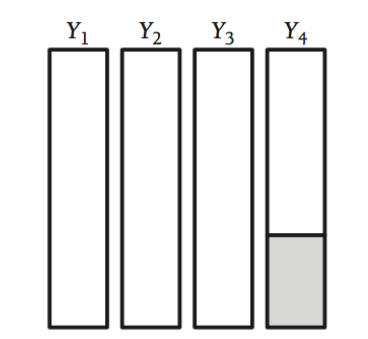
\includegraphics[width=7cm]{1.png}

\begin{definition}[Monotone pattern]
    A missing data pattern is called \textbf{monotone} if the dataset can be arranged by
sorting rows and/or columns such that going from left to rights if a missing
value occurs in a row, all the following values in that row are missing as
well.
\end{definition}

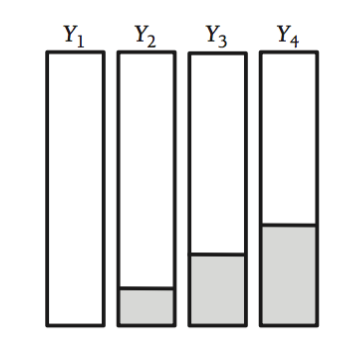
\includegraphics[width=7cm]{2.png}

\begin{itemize}
    \item A monotone pattern resembles a staircase. 
    \item A monotone missing data pattern is typically associated with a
        longitudinal study were participants drop out and never return.
    \item E.g. Consider a clinical trial for a new medication in which
        participants quit the study b.c they are having adverse reactions to
        the drug.
\end{itemize}



\begin{definition}[Arbitrary/General Pattern]
    An \textbf{arbitrary/general} pattern in which any set of variables may
    be missing for any subject is shown in the figure below.
\end{definition}

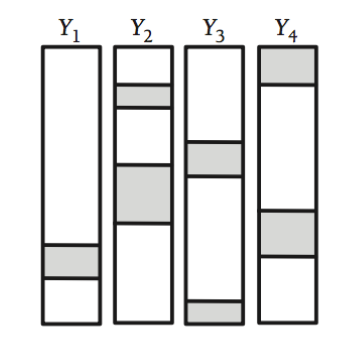
\includegraphics[width=7cm]{3.png}

\begin{itemize}
    \item This pattern corresponds to the most common configuration of
        missing data and cannot be reduced to a univariate or monotone
        pattern.
    \item As a simple example, consider again the two variable example
        involving the number of children living in a household and hourly
        wage. The missing data pattern would be arbitrary if for some households
        the number of children is missing but hourly wage is observed and in
        contrast, for other households the number of children is observed
        but hourly wage is missing.
\end{itemize}




\section{Formal Description of the missing data mechanisms}

\subsection{Notation and terminology}

\begin{definition}[Complete Data]
    The complete data consists of the values one would have obtained if there
    were no missing data and we denote it by $\mathbb{Y}$.
\\ The complete data is partially a hypothetical entity b.c some of its values
might be missing.
\\ we write $Y = (Y_{obs}, Y_{mis})$,
    where they denote the observed components and the missing components of
    $Y$, respectively.
\begin{itemize}
    \item Let $R$ be the missingness indicator. Assuming $\mathbb{Y}
        \in \mathbb{R}^{n\times p}$, where $n$ is the number of subjects and
        $p$ is the number of variables, $R$ has also dimension $n \times p$
        and it is defined as:
\begin{equation}
R_{i j}= \begin{cases}1 & \text { if } Y_{i j} \text { has been observed } \\ 0 & \text { if } Y_{i j} \text { is missing }\end{cases}
\end{equation}
    \item The missing data model is a model for the conditional
        distribution of $R$ given $Y$. Let $f(r|y,\phi)$ denote the probability
        that $R = r$ given that $Y=y$ according to this model, where $\phi$ is
        an unknown parameter. Here $r$ and $y$ are particular values that
        might be taken by $R$ and $Y$.
\end{itemize}

\end{definition}



\begin{definition}[MCAR]
    Data are said to be MCAR if:
    \begin{equation}
f(\mathbf{r} \mid \mathbf{y}, \boldsymbol{\psi})=f(\mathbf{r} \mid
\boldsymbol{\psi}), \quad \forall \mathbf{y}, \boldsymbol{\psi},
\end{equation}
i.e. under MCAR the missing model is completely unrelated to the data, observed
or missing. It only depends on some parameter $\phi$, the overall probability of
missingness.
\begin{itemize}
    \item The essential feature of MCAR is that the observed data can be
        thought of as a random sample of the complete data.
    \item The validity of MCAR can be checked from the data at hand against
        the alternative MAR, but we can never rule out MNAR.
    \end{itemize}
\end{definition}




\begin{definition}[MAR]
    Data are said to be MAR if:
    \begin{equation}
f(\mathbf{r} \mid \mathbf{y}, \boldsymbol{\psi})=f\left(\mathbf{r} \mid \mathbf{y}_{\text {obs }}, \psi\right), \quad \forall \mathbf{y}_{\text {mis }}, \psi
\end{equation}
i.e. under MAR the probability of the pattern of missing data only depends on
the observed data.
\begin{itemize}
    \item Within strata defined by $Y_{obs}$, missingness is MCAR.
    \item The validity of the MAR assumption cannot be checked from the data
        at hand against MNAR.
    \end{itemize}
\end{definition}



\begin{definition}[MNAR]
    Data are said to be MNAR if:
    \begin{equation}
f(\mathbf{r} \mid \mathbf{y}, \boldsymbol{\psi})=f\left(\mathbf{r} \mid \mathbf{y}_{\mathrm{obs}}, \mathbf{y}_{\mathrm{mis}}, \boldsymbol{\psi}\right), \quad \forall \boldsymbol{\psi}
\end{equation}
i.e. the probability of the missing data pattern depends on the unobserved data
and may depend also on the observed ones.
\begin{itemize}
    \item A complicated form of MNAR is when missingness depends on a
        completely unobserved/unmeasured variable.
    \item For the BMI/glucose example, suppose that the true missing mechanism
        for BMI is MAR, hence meaning that individuals with missing values of
        BMI may be more likely to have extreme blood glucose levels.
        However, the MAR missing values in BMI would become MNAR if we had
        no measurements of glucose at all.

    \end{itemize}
\end{definition}



\subsection{Ignorability versus nonignorability}
\begin{itemize}
    \item The $\psi$ parameter of the missing data model have no scientific interest (e.g., had the data been complete there would be no reason to worry about $\psi$ ) and is generally unknown.
    \item It would greatly simplify the analysis if we could just ignore this parameter. However, in some situations, this parameter may influence the estimate of the parameter of interest, the parameter, say $\boldsymbol{\theta}$, of the data model $f(\mathbf{y} \mid \boldsymbol{\theta})$.
    \item The practical importance of Rubin's distinction between MCAR, MAR, and MNAR is that it clarified the conditions that need to exist in order to accurately estimate $\boldsymbol{\theta}$ without the need to know $\psi$.
    \item Rubin showed that likelihood based analyses (e.g., maximum likelihood) and multiple imputation do not require information about $\psi$ if:
(1) the data are MAR or MCAR, and
(2) the parameters $\boldsymbol{\theta}$ and $\psi$ are distinct, in the sense that the joint parameter space of $(\psi, \theta)$ is the product of the parameter space of $\psi$ and the parameter space of $\theta$.
\item Schafer (1997, p.11) says that in many situations the second condition is, at least, reasonable from an intuitive point of view, given that knowing $\theta$ will provide little information about $\psi$ and vice-versa.
\item For this reason, missing data literature often describes MAR (and MCAR!) data as ignorable. Although strictly speaking, we still need (2), not only (1). We will study this more carefully later in the course.
\end{itemize}
\end{definition}

\subsection{Checking MCAR v.s. MAR}
\begin{itemize}
    \item One popular and simple option is to perform $t-tests$. This approach
        seperates the missing and observed values on a particular variable
        and uses t-test to examine group mean differences in the two groups
        induced by such splitting in the other variables in the dataset.
\item The MCAR mechanism implies that such two groups should be similar on average.
\item As a consequence, a non significant t-test (i.e., not rejecting the null hypothesis that the
means of the two groups are equal) provides evidence that data can be MCAR .
\item The main advantage for implementing the t-test approach is to identify (auxiliar) variables
that we can later adjust for in the missing data handling procedure, or
alternaitvely use density plots and boxplots to visualise the
distributions of the two groups.
\item As the number of variables grow, computing the t-test statistics can be
    cumbersome.
\end{itemize}


\subsection{Prevent MNAR missingness}
\begin{itemize}
    \item The ideal solution to the missing data problem would be to have
none.
\item Most of the methods we will cover assume MAR data. However, we cannot be sure
whether the data are really missing at random, or whether the missingness depends on
unobserved variables or the missing data themselves.
\item The idea is to start the study with a data collection strategy that will turn MNAR
missingness into MAR missingness.
\item This, so called inclusive analysis strategy, incorporates variables that are known to be
correlated with the missing prone variables. Then, missing values will be more likely to be
MAR than MNAR.
\item These correlates variables are called auxiliary variables in the missing
    data literature. \\ Note that auxiliary variables might not be of substantial interest in the sense that they
would not have been included in the analysis had the data been complete. \\ Note that the inclusion of auxiliary variables per se does not guarantee that the MAR
assumption is satisfied, but it certainly improves the chances of it. \\ For instance, it may be a strong assumption that nonresponse to an income question in a
survey depends only on gender, race and education, but this is certainly a lot more
plausible than assuming the probability of nonresponse is constant, or that it depends only
on one of these variables.


\end{itemize}























\end{document}
